% Options for packages loaded elsewhere
\PassOptionsToPackage{unicode}{hyperref}
\PassOptionsToPackage{hyphens}{url}
\PassOptionsToPackage{dvipsnames,svgnames,x11names}{xcolor}
%
\documentclass[
  letterpaper,
  DIV=11,
  numbers=noendperiod]{scrreport}

\usepackage{amsmath,amssymb}
\usepackage{iftex}
\ifPDFTeX
  \usepackage[T1]{fontenc}
  \usepackage[utf8]{inputenc}
  \usepackage{textcomp} % provide euro and other symbols
\else % if luatex or xetex
  \usepackage{unicode-math}
  \defaultfontfeatures{Scale=MatchLowercase}
  \defaultfontfeatures[\rmfamily]{Ligatures=TeX,Scale=1}
\fi
\usepackage[]{urw-garamond}
\ifPDFTeX\else  
    % xetex/luatex font selection
\fi
% Use upquote if available, for straight quotes in verbatim environments
\IfFileExists{upquote.sty}{\usepackage{upquote}}{}
\IfFileExists{microtype.sty}{% use microtype if available
  \usepackage[]{microtype}
  \UseMicrotypeSet[protrusion]{basicmath} % disable protrusion for tt fonts
}{}
\makeatletter
\@ifundefined{KOMAClassName}{% if non-KOMA class
  \IfFileExists{parskip.sty}{%
    \usepackage{parskip}
  }{% else
    \setlength{\parindent}{0pt}
    \setlength{\parskip}{6pt plus 2pt minus 1pt}}
}{% if KOMA class
  \KOMAoptions{parskip=half}}
\makeatother
\usepackage{xcolor}
\setlength{\emergencystretch}{3em} % prevent overfull lines
\setcounter{secnumdepth}{3}
% Make \paragraph and \subparagraph free-standing
\ifx\paragraph\undefined\else
  \let\oldparagraph\paragraph
  \renewcommand{\paragraph}[1]{\oldparagraph{#1}\mbox{}}
\fi
\ifx\subparagraph\undefined\else
  \let\oldsubparagraph\subparagraph
  \renewcommand{\subparagraph}[1]{\oldsubparagraph{#1}\mbox{}}
\fi


\providecommand{\tightlist}{%
  \setlength{\itemsep}{0pt}\setlength{\parskip}{0pt}}\usepackage{longtable,booktabs,array}
\usepackage{calc} % for calculating minipage widths
% Correct order of tables after \paragraph or \subparagraph
\usepackage{etoolbox}
\makeatletter
\patchcmd\longtable{\par}{\if@noskipsec\mbox{}\fi\par}{}{}
\makeatother
% Allow footnotes in longtable head/foot
\IfFileExists{footnotehyper.sty}{\usepackage{footnotehyper}}{\usepackage{footnote}}
\makesavenoteenv{longtable}
\usepackage{graphicx}
\makeatletter
\def\maxwidth{\ifdim\Gin@nat@width>\linewidth\linewidth\else\Gin@nat@width\fi}
\def\maxheight{\ifdim\Gin@nat@height>\textheight\textheight\else\Gin@nat@height\fi}
\makeatother
% Scale images if necessary, so that they will not overflow the page
% margins by default, and it is still possible to overwrite the defaults
% using explicit options in \includegraphics[width, height, ...]{}
\setkeys{Gin}{width=\maxwidth,height=\maxheight,keepaspectratio}
% Set default figure placement to htbp
\makeatletter
\def\fps@figure{htbp}
\makeatother

\KOMAoption{captions}{tableheading}
\makeatletter
\@ifpackageloaded{tcolorbox}{}{\usepackage[skins,breakable]{tcolorbox}}
\@ifpackageloaded{fontawesome5}{}{\usepackage{fontawesome5}}
\definecolor{quarto-callout-color}{HTML}{909090}
\definecolor{quarto-callout-note-color}{HTML}{0758E5}
\definecolor{quarto-callout-important-color}{HTML}{CC1914}
\definecolor{quarto-callout-warning-color}{HTML}{EB9113}
\definecolor{quarto-callout-tip-color}{HTML}{00A047}
\definecolor{quarto-callout-caution-color}{HTML}{FC5300}
\definecolor{quarto-callout-color-frame}{HTML}{acacac}
\definecolor{quarto-callout-note-color-frame}{HTML}{4582ec}
\definecolor{quarto-callout-important-color-frame}{HTML}{d9534f}
\definecolor{quarto-callout-warning-color-frame}{HTML}{f0ad4e}
\definecolor{quarto-callout-tip-color-frame}{HTML}{02b875}
\definecolor{quarto-callout-caution-color-frame}{HTML}{fd7e14}
\makeatother
\makeatletter
\makeatother
\makeatletter
\@ifpackageloaded{bookmark}{}{\usepackage{bookmark}}
\makeatother
\makeatletter
\@ifpackageloaded{caption}{}{\usepackage{caption}}
\AtBeginDocument{%
\ifdefined\contentsname
  \renewcommand*\contentsname{Innehåll}
\else
  \newcommand\contentsname{Innehåll}
\fi
\ifdefined\listfigurename
  \renewcommand*\listfigurename{Figurlista}
\else
  \newcommand\listfigurename{Figurlista}
\fi
\ifdefined\listtablename
  \renewcommand*\listtablename{Tabellista}
\else
  \newcommand\listtablename{Tabellista}
\fi
\ifdefined\figurename
  \renewcommand*\figurename{Figur}
\else
  \newcommand\figurename{Figur}
\fi
\ifdefined\tablename
  \renewcommand*\tablename{Tabell}
\else
  \newcommand\tablename{Tabell}
\fi
}
\@ifpackageloaded{float}{}{\usepackage{float}}
\floatstyle{ruled}
\@ifundefined{c@chapter}{\newfloat{codelisting}{h}{lop}}{\newfloat{codelisting}{h}{lop}[chapter]}
\floatname{codelisting}{Listing}
\newcommand*\listoflistings{\listof{codelisting}{List of Listings}}
\makeatother
\makeatletter
\@ifpackageloaded{caption}{}{\usepackage{caption}}
\@ifpackageloaded{subcaption}{}{\usepackage{subcaption}}
\makeatother
\makeatletter
\@ifpackageloaded{tcolorbox}{}{\usepackage[skins,breakable]{tcolorbox}}
\makeatother
\makeatletter
\@ifundefined{shadecolor}{\definecolor{shadecolor}{rgb}{.97, .97, .97}}
\makeatother
\makeatletter
\makeatother
\makeatletter
\makeatother
\ifLuaTeX
  \usepackage{selnolig}  % disable illegal ligatures
\fi
\IfFileExists{bookmark.sty}{\usepackage{bookmark}}{\usepackage{hyperref}}
\IfFileExists{xurl.sty}{\usepackage{xurl}}{} % add URL line breaks if available
\urlstyle{same} % disable monospaced font for URLs
\hypersetup{
  pdftitle={KM3},
  colorlinks=true,
  linkcolor={blue},
  filecolor={Maroon},
  citecolor={Blue},
  urlcolor={Blue},
  pdfcreator={LaTeX via pandoc}}

\title{KM3}
\author{}
\date{2023-09-07}

\begin{document}
\maketitle
\ifdefined\Shaded\renewenvironment{Shaded}{\begin{tcolorbox}[breakable, boxrule=0pt, interior hidden, sharp corners, enhanced, borderline west={3pt}{0pt}{shadecolor}, frame hidden]}{\end{tcolorbox}}\fi

\renewcommand*\contentsname{Innehåll}
{
\hypersetup{linkcolor=}
\setcounter{tocdepth}{2}
\tableofcontents
}
\bookmarksetup{startatroot}

\hypertarget{preface}{%
\chapter*{Preface}\label{preface}}
\addcontentsline{toc}{chapter}{Preface}

\markboth{Preface}{Preface}

\bookmarksetup{startatroot}

\hypertarget{introduction}{%
\chapter{Introduction}\label{introduction}}

This is a book created from markdown and executable code.

See @knuth84 for additional discussion of literate programming.

\part{Ortopedi}

\hypertarget{allmuxe4n-frakturluxe4ra}{%
\chapter{Allmän frakturlära}\label{allmuxe4n-frakturluxe4ra}}

\begin{tcolorbox}[enhanced jigsaw, colback=white, colbacktitle=quarto-callout-warning-color!10!white, toptitle=1mm, arc=.35mm, toprule=.15mm, rightrule=.15mm, titlerule=0mm, breakable, bottomrule=.15mm, colframe=quarto-callout-warning-color-frame, left=2mm, opacityback=0, coltitle=black, title=\textcolor{quarto-callout-warning-color}{\faExclamationTriangle}\hspace{0.5em}{Riskfaktorer}, leftrule=.75mm, bottomtitle=1mm, opacitybacktitle=0.6]

\begin{itemize}
\tightlist
\item
  Hög ålder
\item
  Kvinna
\item
  Rökning
\item
  Osteoporos
\item
  Ökad fallrisk
\end{itemize}

\end{tcolorbox}

\hypertarget{klassifikation}{%
\section{Klassifikation}\label{klassifikation}}

Hos vuxna anses allt som inte är diafysärt som metafysärt. Begreppet
epifys används därför endast hos barn med öppna fyser!\\
\textbf{End segment} = Område lika långt som den bredaste delen av
benet\\
\textbf{Mid segment} = resten

Klassifikationer inkluderar:

\begin{itemize}
\tightlist
\item
  \textbf{Grad av våld}

  \begin{itemize}
  \tightlist
  \item
    Lågenergiskada --- Ofta i samband med osteoporos
  \item
    Högenergiskada
  \end{itemize}
\item
  \textbf{Anatomisk lokalisation}

  \begin{itemize}
  \tightlist
  \item
    Axial vs appendikulär fraktur
  \item
    \textbf{Specifik lokal} --- Har betydelse för läkning och prognos

    \begin{itemize}
    \tightlist
    \item
      Diafysär
    \item
      Metafysär --- Läker snabbare än diafysär
    \item
      Fysär --- Tillväxtzon hos barn, kan ge tillväxtstörning
    \item
      Epifysär --- Kan ge tillväxtstörning om frakturen går in i fysen\\
      Begreppet används inte om \emph{fysen} slutits.
    \item
      Intraartikulär --- Engagerar led
    \item
      Extraartikulär --- Engagerar ej led
    \item
      Epikondylär
    \item
      Kondylär\\
    \item
      Subkapitulär
    \item
      Suprakondylär
    \item
      Transkondylär
    \item
      Ligamentavulsion --- Bendel med ligamentfäste slits av
    \item
      Apofysavulsion --- Ger ej tillväxtfel.
    \item
      \textbf{Höftfrakturer}

      \begin{itemize}
      \tightlist
      \item
        Cervikal --- Genom \emph{collum femoris}.
      \item
        Pertokantär --- Genom \emph{trochanter minor/major}.
      \item
        Subtrokantär --- Från \emph{trochanter minor} tom 5cm distalt om
        denna.
      \end{itemize}
    \end{itemize}
  \end{itemize}
\item
  \textbf{Utseende}

  \begin{itemize}
  \tightlist
  \item
    Longitudinell
  \item
    Transversell
  \item
    Spiralfraktur
  \item
    Kompressionsfraktur
  \item
    Komminut (5=kompression av tillväxtzonen)
  \item
    Patologisk --- t.ex tumör, hereditär sjukdom
  \item
    Stressfraktur --- uppstår vid återkommande belastning under tid, kan
    progrediera till ``riktig'' fraktur
  \end{itemize}
\item
  \textbf{Mjukdelsskada}

  \begin{itemize}
  \tightlist
  \item
    Öppna vs slutna
  \end{itemize}
\end{itemize}

\hypertarget{klassifikation-hos-barn}{%
\subsection{Klassifikation hos barn}\label{klassifikation-hos-barn}}

Skiljs från vuxna då barns tjocka periostie och mjuka skellett ofta ger
annan bild.

\begin{itemize}
\tightlist
\item
  Böjningsfraktur
\item
  Inkomplett Kompressionsfraktur (\emph{torus}-fraktur)
\item
  Inkomplett gångjärnsfraktur (\emph{greenstick}-fraktur)
\item
  Komplett fraktur --- Vanligare hos äldre barn
\item
  \textbf{Utifrån lokal jmf tillväxtzon}

  \begin{itemize}
  \tightlist
  \item
    Salter-harris 1-5\\
    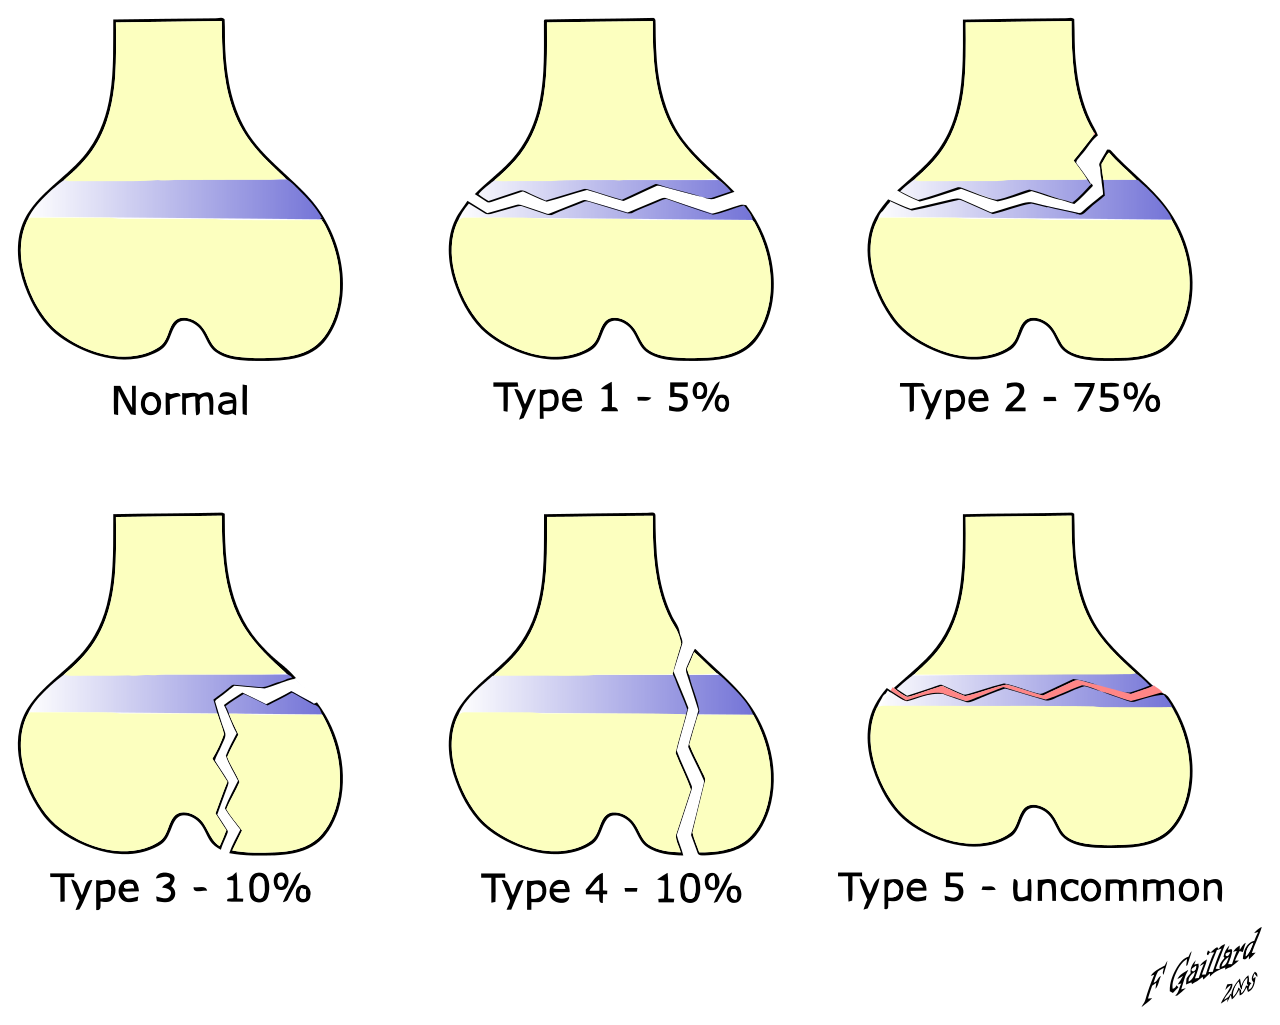
\includegraphics[width=0.5\textwidth,height=0.5\textheight]{pics/1280px-SalterHarris.svg.png}
  \end{itemize}
\end{itemize}

\hypertarget{frakturluxe4kning}{%
\section{Frakturläkning}\label{frakturluxe4kning}}

Det finns principiellt 2 typer av läkningar:\\
\textbf{1.} Direkt läkning utan synlig kallus\\
\textbf{2.} Indirekt läkning med kallus\\
Läkningstyp beror på huruvida (icke-splittrade) frakturer blir stabilt
anatomiskt reponerade.

\hypertarget{intern-fixation}{%
\subsection{Intern fixation}\label{intern-fixation}}

Åstadkoms ofta med skenor av rostfritt stål\footnote{Legering av järn,
  krom, nickel eller kobolt-kromolybden-legering}.\\
Märgspikar består oftast av titan som är mer elastiskt och bildar ett
bakteriedödande oxidlager.\\
På ställen med låg belastning kan resorberbara implantat av polyestrar
användas.

\hypertarget{uxf6vre-extremiteten}{%
\chapter{Övre extremiteten}\label{uxf6vre-extremiteten}}

\hypertarget{uxf6verarmen}{%
\section{Överarmen}\label{uxf6verarmen}}

\hypertarget{diafysuxe4r-humerusfraktur}{%
\subsection{Diafysär humerusfraktur}\label{diafysuxe4r-humerusfraktur}}

Uppstår \textbf{oftast} till följd av direkt våld men ses även vid t.ex
armbrytning och polisgrepp.\\
Eventuell felställning beror på frakturens lokal. Distala och proximala
frakturer ger ofta mer felställning pga muskelfästen som drar i
fragment.

\begin{tcolorbox}[enhanced jigsaw, colback=white, colbacktitle=quarto-callout-tip-color!10!white, toptitle=1mm, arc=.35mm, toprule=.15mm, rightrule=.15mm, titlerule=0mm, breakable, bottomrule=.15mm, colframe=quarto-callout-tip-color-frame, left=2mm, opacityback=0, coltitle=black, title=\textcolor{quarto-callout-tip-color}{\faLightbulb}\hspace{0.5em}{Klassifikation}, leftrule=.75mm, bottomtitle=1mm, opacitybacktitle=0.6]

Görs enl. AO/OTA och delas in i ABC samt grad 1-3:\\
\textbf{A} --- 2-fragmentsfrakturer\\
\textbf{B} --- 3-fragmentsfrakturer\\
\textbf{C} --- Komminutfrakturer

Siffra (1-3) beror på svårighetsgrad.

\end{tcolorbox}

\emph{N. radialis}påverkan är relativt vanligt då nerven går nära
diafysen. Även tryck från hematom och gips kan påverka den! De flesta
radialispareser är dock övergående.

\hypertarget{kliniska-dragdiagnos}{%
\paragraph{Kliniska drag/Diagnos}\label{kliniska-dragdiagnos}}

Fraktur bör misstänkas hos en patient som klagar på smärta/nedsatt
rörelseförmåga i överarmen efter trauma.

Vid undersökning ses ofta direkt/indirekt smärta, felställning och
frakturkrepetationer.\\
\textbf{Distalstatus} ska alltid ingå i undersökningen!

Diagnosen bekräftas med röntgen av hela humerus.

\hypertarget{behandling}{%
\paragraph{Behandling}\label{behandling}}

Som regel kan diafysära humerusfrakturer behandlas konservativt.\\
Gipsskena samt ortos och slynga kombinerat med armens egen vikt kan ofta
hålla den rät och hindra felställning samt förkortning.\\
Efter ca 4 veckor med gips kan slutbehandling ske med ortos som omsluter
humerus.

\textbf{Indikationer för kirurgi är:}

\begin{itemize}
\tightlist
\item
  Vinkelfelställning \textgreater{} 20 grader
\item
  Förkortning \textgreater{} 3cm
\item
  Öppen fraktur
\item
  Kärlskador
\item
  Multipla frakturer (Där kirurgisk stabilisering underlättar
  mobilisering)
\item
  Patologisk fraktur
\item
  \emph{Non-union} av äldre fraktur
\end{itemize}

Operativ behandling är oftast märgspik eller plattfixation.

Vid radialispares efter sluten fraktur kan nervfunktion väntas återkomma
inom 3 månader. Explorativ kirurgi utförs endast efter denna tidsgräns
samt neurofysiologisk undersökning (Görs \emph{alltid} öppen fraktur som
opereras).

\hypertarget{prognos}{%
\paragraph{Prognos}\label{prognos}}

Läker i genomsnitt på 12v.\\
Långa och sneda frakturer(inkl. komminut) läker bättre än korta,
tvära.\\
\textless10\% kräver kirugisk behandling. Är frakturen rörlig efter
\textbf{4 månader} klassas den som \emph{non-union}.

\hypertarget{armbuxe5gen}{%
\section{Armbågen}\label{armbuxe5gen}}

\hypertarget{sec-olekranonfraktur}{%
\subsection{Olekranonfraktur}\label{sec-olekranonfraktur}}

Olekranonfrakturer ingår i proximala ulnafrakturer tillsammans med
Koronoidfraktur (Kapitel~\ref{sec-koronoidfraktur}) och proximal
skaftfraktur. Dessa uppkommer oftare tillsammans med andra skador
jämfört med olekranonfrakturer.

\begin{tcolorbox}[enhanced jigsaw, colback=white, colbacktitle=quarto-callout-tip-color!10!white, toptitle=1mm, arc=.35mm, toprule=.15mm, rightrule=.15mm, titlerule=0mm, breakable, bottomrule=.15mm, colframe=quarto-callout-tip-color-frame, left=2mm, opacityback=0, coltitle=black, title=\textcolor{quarto-callout-tip-color}{\faLightbulb}\hspace{0.5em}{Klassifikation}, leftrule=.75mm, bottomtitle=1mm, opacitybacktitle=0.6]

\begin{itemize}
\tightlist
\item
  \textbf{Extraartikulära} --- ca 10\%, proximal avulsionsfraktur
  (\textasciitilde avlösning av triceps)
\item
  \textbf{Intraartikulära} --- Indelas enl. Morrey

  \begin{itemize}
  \tightlist
  \item
    Typ I --- Odislocerad
  \item
    Typ II --- Dislocerad, stabil
  \item
    Typ III --- Dislocerad, instabil

    \begin{itemize}
    \tightlist
    \item
      Utgör ca 15\% av fall. Engagerar \emph{proc. coronoideus} och
      kollateralligament, \textbf{mycket instabil}.
    \end{itemize}
  \end{itemize}
\end{itemize}

\end{tcolorbox}

\hypertarget{kliniska-dragdiagnos-1}{%
\paragraph{Kliniska drag/Diagnos}\label{kliniska-dragdiagnos-1}}

Som vid andra armbågsfrakturer. Pat. saknar förmåga att extendera i
armbågsleden. Röntgen bekräftar diagnos.

\hypertarget{behandling-1}{%
\paragraph{Behandling}\label{behandling-1}}

\textbf{Odislocerad typ I-fraktur:} Gips i 3 veckor. En dislocering på
ett par mm medför behov av operation!\\
\textbf{Typ II-fraktur:} Kan behandlas konservativt hos patient med
låga-måttliga funktionskrav. (Dvs saknar behov av att aktivt extendera
armbågen)\\
\textbf{Typ III-fraktur:} Opereras \emph{alltid} med reposition och
fixation. Cerklage, eller stift+cerklage och platta kan användas.

\hypertarget{prognos-1}{%
\paragraph{Prognos}\label{prognos-1}}

Med adekvat behandling ses ofta god funktion efter läkning med viss
kvarstående rörelseinskränkning (ffa i extension).

\hypertarget{sec-koronoidfraktur}{%
\subsection{Koronoidfraktur}\label{sec-koronoidfraktur}}

TODO: detta

\begin{tcolorbox}[enhanced jigsaw, colback=white, colbacktitle=quarto-callout-tip-color!10!white, toptitle=1mm, arc=.35mm, toprule=.15mm, rightrule=.15mm, titlerule=0mm, breakable, bottomrule=.15mm, colframe=quarto-callout-tip-color-frame, left=2mm, opacityback=0, coltitle=black, title=\textcolor{quarto-callout-tip-color}{\faLightbulb}\hspace{0.5em}{Klassifikation}, leftrule=.75mm, bottomtitle=1mm, opacitybacktitle=0.6]

Enl. Reagan \& Morrey

\textbf{Typ I:} Endast spetsen av \emph{proc. coronoideus} avlöst.\\
\textbf{Typ II:} Frakturen omfattar \textless50\% av \emph{prc.
coronoideus}.\\
\textbf{Typ IIIA:} \textgreater50\% av \emph{proc. coronoideus}
\textbf{utan} luxation.\\
\textbf{Typ IIIB:} \textgreater50\% av \emph{proc. coronoideus}
\textbf{med} luxation.

\end{tcolorbox}

\hypertarget{kliniska-dragdiagnos-2}{%
\paragraph{Kliniska drag/Diagnos}\label{kliniska-dragdiagnos-2}}

Undersök, luxation? \textbf{Distalstatus!}

\hypertarget{behandling-2}{%
\paragraph{Behandling}\label{behandling-2}}

\textbf{Typ I och II:} Inget gips, ortos eller slynga. Rörelseträning!\\
\textbf{Typ III:} A -\textgreater{} Oftast kirurgisk behandling, B
-\textgreater{} Alltid kirurgisk behandling. Reponering och fixation med
(oftast) skruv. Se även kapitel~\ref{sec-armbågsluxation}

\hypertarget{sec-armbuxe5gsluxation}{%
\subsection{Armbågsluxation}\label{sec-armbuxe5gsluxation}}

\hypertarget{kliniska-dragdiagnos-3}{%
\paragraph{Kliniska drag/Diagnos}\label{kliniska-dragdiagnos-3}}

Undersök armen, distalstatus med särskilt fokus på \emph{n.~ulnaris}.
Slätröntgen bekräftar diagnos och eventuell samtidig fraktur.

\hypertarget{behandling-3}{%
\paragraph{Behandling}\label{behandling-3}}

Om samtidig fraktur krävs ev. operation.

Om ej fraktur föreligger reponeras dorsal luxation enligt:

\begin{enumerate}
\def\labelenumi{\arabic{enumi}.}
\tightlist
\item
  Smärtlindra, morfin 5mg, midazolam 0.5-1mg\\
\item
  Håll armbågen flekterad i 45 grader, dra i underarm samtidigt som
  överarmen hålls still av assistent

  \begin{itemize}
  \tightlist
  \item
    Om ovanstående misslyckas kan man trycka med tummar mot olekranån
    från dorsalsidan.
  \end{itemize}
\item
  Undersök efter reponering:

  \begin{itemize}
  \tightlist
  \item
    Distalstatus
  \item
    Kontrollera stabilitet: extendera, flektera, pronera och supinera.
    Om allt (även passiv extension) kan göras utan reluxation är
    armbågen stabil.
  \end{itemize}
\item
  Gipsa --- Lång, dorsal skena, 90-100grader i armbågen med lite
  pronation.
\item
  Återbesök efter 1 vecka

  \begin{itemize}
  \tightlist
  \item
    Kontrollröntgen, avgipsning, stabilitetskontroll. Om instabilitet
    föreligger gipsas armen på nutt i 2-3 veckor med återbesök därefter.
    Om armen är stabil skrivs remiss till fysioterapeut.\footnote{Undvik
      varus/valgusvackling i 2 månader, töjning i laterala ligament och
      axiell kompression av underarm!}
  \end{itemize}
\end{enumerate}

\hypertarget{prognos-2}{%
\paragraph{Prognos}\label{prognos-2}}

Reluxationer är vanligt, 50\% får kvarvarande rörelseinskränkning.

\hypertarget{underarmen}{%
\section{Underarmen}\label{underarmen}}

\hypertarget{sec-diafysuxe4runderarmsfraktur}{%
\subsection{Diafysär
underarmsfraktur}\label{sec-diafysuxe4runderarmsfraktur}}

\begin{tcolorbox}[enhanced jigsaw, colback=white, colbacktitle=quarto-callout-tip-color!10!white, toptitle=1mm, arc=.35mm, toprule=.15mm, rightrule=.15mm, titlerule=0mm, breakable, bottomrule=.15mm, colframe=quarto-callout-tip-color-frame, left=2mm, opacityback=0, coltitle=black, title=\textcolor{quarto-callout-tip-color}{\faLightbulb}\hspace{0.5em}{Klassifikation}, leftrule=.75mm, bottomtitle=1mm, opacitybacktitle=0.6]

Enligt AO/OTA:\\
\textbf{A}: Enkla tvågragmentsfrakturer\\
\textbf{B}: Frakturer med fjärilsformat/triangulärt
intermediärfragment\\
\textbf{C}: Komplexa, komminuta frakturer

\end{tcolorbox}

\hypertarget{kliniska-dragdiagnos-4}{%
\paragraph{Kliniska drag/Diagnos}\label{kliniska-dragdiagnos-4}}

Patienter söker med något/några av: smärta, svullnad, rotationssmärta,
felställning.\\
Vid undesökning finns ofta tydliga frakturtecken. \textbf{Distalstatus}
ska alltid ingå!

\hypertarget{behandling-4}{%
\paragraph{Behandling}\label{behandling-4}}

Slutna frakturer utan avvikande distalstatus behandlas med gipsskena och
planerad kirurgi.

Målet med behandling är exakt återställande gällande längd, rotation och
böjning hos radius och ulna.\\
En minimalt dislocerade frakturer kan slutbehandlas med gips men
opereras ofta för att snabba på mobiliseringen.\\
Även isolerad ulnafraktur fixeras i allmänhet med platta.\\
Rörelseträning \emph{kan} i allmänhet påbörjas direkt men gipsskena
används ofta i 2 veckor för smärtlindring.\\
Tyngre belastning undviks tills röntgenologisk läkning nåtts.

\hypertarget{prognos-3}{%
\paragraph{Prognos}\label{prognos-3}}

\textbf{Läkningstiden} är ca 3-4 månader i normalfallet. Armkraften kan
räknas vara nedsatt långt efter skadan. Förutsatt att läkning sker utan
felställning normaliseras funktionen i allmänhet med tid.\\
Vid lägre än 50 graders supination/pronation upplevs ofta begränsningar
i vardagen.

\hypertarget{monteggia-fraktur}{%
\subsection{Monteggia-fraktur}\label{monteggia-fraktur}}

Ulnafraktur där dislokation lett till ligamentskada vilket ger
dislokation hos \emph{caput radii} i radiohumeralleden.\\
Radius kan disloceras ventralt, lateralt eller dorsalt. Klassifikation
sker enligt \emph{Bado}\\
Om även \emph{caput radii} är frakturerat benämns frakturen
monteggiaekvivalent.

\hypertarget{kliniska-dragdiagnos-5}{%
\paragraph{Kliniska drag/Diagnos}\label{kliniska-dragdiagnos-5}}

I princip samma symtom som vid diafysär underarmsfraktur
(Kapitel~\ref{sec-diafysärunderarmsfraktur})\\
\textbf{Röntgen} omfattar armbågsled och handled.

\hypertarget{behandling-5}{%
\paragraph{Behandling}\label{behandling-5}}

\textbf{Alla} monteggiafrakturer behandlas med öppen kirugisk reposition
och fixation. Efter att ulna fixerats reponeras ofta \emph{caput radii}
utan vidare åtgärd. Reparation av ligament behövs då sällan.\\
Vid monteggiaekvivalent fraktur fixeras även \emph{caput radii}.

\hypertarget{prognos-4}{%
\paragraph{Prognos}\label{prognos-4}}

Vid korrekt reposition blir patienten oftast besvärsfri efter läkning
som tar 3-4 månader.

\hypertarget{handled}{%
\section{Handled}\label{handled}}

TODO: Initial handläggning och typer

\hypertarget{distal-radiusfraktur}{%
\subsection{Distal radiusfraktur}\label{distal-radiusfraktur}}

Den vanligaste av alla frakturer. \emph{Allra} vanligast hos barn och
postmenopausala kvinnor men förekommer hos alla.\\
Uppkommer oftast efter fall mot utsträckt hand.\\
Hos barn sker frakturen oftast i anslutning till epifysplattan.

\begin{tcolorbox}[enhanced jigsaw, colback=white, colbacktitle=quarto-callout-tip-color!10!white, toptitle=1mm, arc=.35mm, toprule=.15mm, rightrule=.15mm, titlerule=0mm, breakable, bottomrule=.15mm, colframe=quarto-callout-tip-color-frame, left=2mm, opacityback=0, coltitle=black, title=\textcolor{quarto-callout-tip-color}{\faLightbulb}\hspace{0.5em}{Typer}, leftrule=.75mm, bottomtitle=1mm, opacitybacktitle=0.6]

\begin{itemize}
\tightlist
\item
  \textbf{Colles} --- Vanligast, fraktur genom metafysen med
  dorsalbockat fragment.
\item
  \textbf{Smith} --- Som Colles men volarbockad.
\item
  \textbf{Barton} --- Frakturen löper genom leden.
\item
  \textbf{Chauffeur} --- Avulsion av \emph{proc. styloideus radii}. Kan
  ge allvarliga ligamenskador.
\item
  \textbf{Dye punch} --- Ledytan frakturerar och trycks in mot
  metafysen.
\end{itemize}

\end{tcolorbox}

Kraftigt dorsalbockade frakturer ger alltid skador mot distala
ulna.\footnote{\emph{Proc. styloideus ulnae}-fraktur eller
  ledbandsskador.}

\hypertarget{symtomdiagnos}{%
\paragraph{Symtom/Diagnos}\label{symtomdiagnos}}

Fall mot handen med smärta/svullnad inger misstanke. Även skador i
\emph{ossa carpi} bör övervägas. Rtg bekräftar diagnos.\\
DT kan övervägas vid komminuta frakturer samt vid ledengagemang inför
operation.

\hypertarget{behandling-6}{%
\paragraph{Behandling}\label{behandling-6}}

\textbf{Odislocerad fraktur i ung vuxen utan osteoporos:}\\
Gipsskena i 4-5 veckor, Rtg-kontroll efter 7-10 dagar.

\begin{tcolorbox}[enhanced jigsaw, colback=white, colbacktitle=quarto-callout-warning-color!10!white, toptitle=1mm, arc=.35mm, toprule=.15mm, rightrule=.15mm, titlerule=0mm, breakable, bottomrule=.15mm, colframe=quarto-callout-warning-color-frame, left=2mm, opacityback=0, coltitle=black, title=\textcolor{quarto-callout-warning-color}{\faExclamationTriangle}\hspace{0.5em}{Varning}, leftrule=.75mm, bottomtitle=1mm, opacitybacktitle=0.6]

Chauffeur-fraktur bör kontrolleras efter utläkning även om den är helt
odislocerad!

\end{tcolorbox}

Även något dislocerade frakturer kan gipsas. Frakturer som varit volart
dislocerade kräver volart stöd och vice versa.

Hos en inidivid med höga funktionskrav bör exakt reposition
eftersträvas. Om detta inte kan uppnås med gips är kirurgi ofta
indicerat.

Indikationer för öppen reposition:

\begin{itemize}
\tightlist
\item
  Initial dorsalbockning \textgreater30 grader
\item
  Smiths fraktur
\item
  Intraartikulära frakturer med \textgreater1mm skillnad i ledyte mellan
  fragment
\item
  Frakturer som engagerar \emph{ossa carpi}
\item
  Felställd fraktur med samtidigt dislocerad ulnafraktur
\item
  Bilaterala frakturer
\item
  Frakturer med uttalad instabilitet kring distala ulnaänden.
\end{itemize}

Hos individer med låga funktionskrav är operation sällan indicerad.

\hypertarget{prognos-5}{%
\paragraph{Prognos}\label{prognos-5}}

Prognos efter okomplicerad fraktur/läkning är god. Höga funktionskrav
och komplex fraktur ökar risk för bestående kliniskt relevanta symtom.

\begin{tcolorbox}[enhanced jigsaw, colback=white, colbacktitle=quarto-callout-warning-color!10!white, toptitle=1mm, arc=.35mm, toprule=.15mm, rightrule=.15mm, titlerule=0mm, breakable, bottomrule=.15mm, colframe=quarto-callout-warning-color-frame, left=2mm, opacityback=0, coltitle=black, title=\textcolor{quarto-callout-warning-color}{\faExclamationTriangle}\hspace{0.5em}{Complex Regional Pain Syndrome}, leftrule=.75mm, bottomtitle=1mm, opacitybacktitle=0.6]

\textbf{CPRS} ger uttalad svullnad av handen, känselstörning, förändrad
temperaturreglering och ökad behåring.\\
Risken ökar med långvarig immobilisering.

\end{tcolorbox}

\hypertarget{skafoideumfraktur}{%
\subsection{Skafoideumfraktur}\label{skafoideumfraktur}}

Den vanligaste frakturen bland \emph{ossa carpi}.

\hypertarget{kliniska-dragdiagnos-6}{%
\paragraph{Kliniska drag/Diagnos}\label{kliniska-dragdiagnos-6}}

Bör misstänkas hos samma grupp som ovan.

Kliniska tecken:

\begin{enumerate}
\def\labelenumi{\arabic{enumi}.}
\tightlist
\item
  Palpationsöm i \emph{fossa tabatiére}
\item
  Palpationsöm över \emph{tuberositas scaphoideum}
\item
  Ömhet vid axialkompression av tumme
\item
  Ömhet vid radialdeviation handled
\end{enumerate}

\textbf{Diagnos} ges via röntgen där skafoideumprojektioner bör
begäras.\\
Vid negativt röntgenutfall men klinisk bild som pekar mot fraktur bör
skafoideumgips sättas och röntgen göras om efter en vecka. MR kan ofta
påvisa fraktur snabbare än rtg i dessa fall.

\hypertarget{behandling-7}{%
\paragraph{Behandling}\label{behandling-7}}

\begin{itemize}
\tightlist
\item
  \textbf{Avulsionsfraktur av tuberositas scaphoideum:}

  \begin{itemize}
  \tightlist
  \item
    Elastisk linda, avtagning i hemmet efter 2v.
  \end{itemize}
\item
  \textbf{Odislocerad proximal-/midjefraktur:}

  \begin{itemize}
  \tightlist
  \item
    Skafoideumgips, återbesök efter 4v. Undvik riskbelastning i 2v efter
    avgipsning.
  \end{itemize}
\item
  \textbf{Dislocerad proximal-/midjefraktur(\textgreater1mm):}

  \begin{itemize}
  \tightlist
  \item
    Oftast skruvfixation.
  \end{itemize}
\end{itemize}

\hypertarget{prognos-6}{%
\paragraph{Prognos}\label{prognos-6}}

Sämre ju mer proximal fraktur. Opererade frakturer läker i allmänhet
komplikationsfritt.

\hypertarget{uxf6vriga-ossa-carpi}{%
\subsection{\texorpdfstring{Övriga \emph{ossa
carpi}}{Övriga ossa carpi}}\label{uxf6vriga-ossa-carpi}}

TODO: Detta

\hypertarget{karpal-luxationinstabilitet}{%
\subsection{Karpal
luxation/instabilitet}\label{karpal-luxationinstabilitet}}

Alltid resultat av högenergitrauma.

\hypertarget{kliniska-dragdiagnos-7}{%
\paragraph{Kliniska drag/Diagnos}\label{kliniska-dragdiagnos-7}}

Smärta, svullnad, felställning i handleden.\\
\emph{N. medianus} är ofta påverkad.\\
Dessa skador är inte sällan svårupptäckta röntgenologiskt. DT kan här
komplettera diagnostiken.

\hypertarget{behandling-8}{%
\paragraph{Behandling}\label{behandling-8}}

Perilunär luxation kan (ibland) reponeras slutet men måste fixeras
kirurgiskt. \emph{N. medianus} måste dekomprimeras vid påverkan.

\hypertarget{prognos-7}{%
\paragraph{Prognos}\label{prognos-7}}

Leder alltid till inskränkt rörlighet med stor risk för
artrosutveckling. Snabb handlägnning ger minskad risk för
\emph{n.~medianus}-påverkan.

\hypertarget{de-quervains-tendinit}{%
\subsection{De Quervains tendinit}\label{de-quervains-tendinit}}

Orsakas av svullnad i \emph{abductor pollicis longus}-/\emph{extensor
pollicis brevis}-senan.\\
Detta kan ske vid blödning/trauma och akut tenosynovit. En vanlig
patientgrupp är kvinnor som börjat amma och då \textbf{använder handen
på ett nytt sätt}. Tillståndet kan komma och försvinna relativt
plöstligt.

\hypertarget{kliniska-dragdiagnos-8}{%
\paragraph{Kliniska drag/Diagnos}\label{kliniska-dragdiagnos-8}}

Klinisk diagnos:

\begin{itemize}
\tightlist
\item
  Ömhet över det första dorsala senfacket
\item
  Positivt finkelsteins test
\end{itemize}

\begin{figure}

{\centering 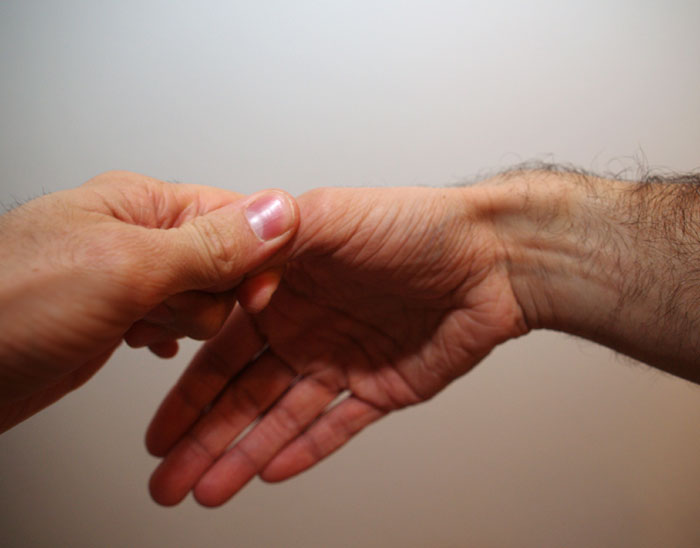
\includegraphics[width=0.5\textwidth,height=\textheight]{pics/Originaler_Finkelstein-Test.jpg}

}

\caption{Finkelsteins test}

\end{figure}

Tumbasartros kan uteslutas mha rtg vid osäkerhet kring diagnos.

\hypertarget{behandling-9}{%
\paragraph{Behandling}\label{behandling-9}}

\begin{itemize}
\tightlist
\item
  Ortos som hindrar tum-/handledsrörelser
\item
  Kortisoninjektion i senskidan
\item
  Vid recidiv/ej tillfredssällande resultat -\textgreater{} operation
\end{itemize}

\hypertarget{prognos-8}{%
\paragraph{Prognos}\label{prognos-8}}

Icke-kirurgisk behandling ger ofta goda resultat. Kirurgi leder nästan
alltid till besvärsfrihet.

\hypertarget{ganglion}{%
\subsection{Ganglion}\label{ganglion}}

TODO: Detta

\hypertarget{lunatummalaci}{%
\subsection{Lunatummalaci}\label{lunatummalaci}}

\hypertarget{skafoideumpseudoartros}{%
\subsection{Skafoideumpseudoartros}\label{skafoideumpseudoartros}}

\hypertarget{skafolunuxe4r-ligamentskada}{%
\subsection{Skafolunär
ligamentskada}\label{skafolunuxe4r-ligamentskada}}

\hypertarget{lunotrikvetral-ligamentskada}{%
\subsection{Lunotrikvetral
ligamentskada}\label{lunotrikvetral-ligamentskada}}

\hypertarget{tfcc-skada}{%
\subsection{TFCC-skada}\label{tfcc-skada}}

\hypertarget{handledsarotros}{%
\subsection{Handledsarotros}\label{handledsarotros}}

\hypertarget{nedre-extremiteten}{%
\chapter{Nedre extremiteten}\label{nedre-extremiteten}}

\hypertarget{buxe4cken}{%
\section{Bäcken}\label{buxe4cken}}

\hypertarget{buxe4ckenfraktur}{%
\subsection{Bäckenfraktur}\label{buxe4ckenfraktur}}

Sker i princip antingen vid osteoporostillstånd+lågenergivåld eller hos
unga efter högenergivåld. Efter lågenergivåld är de nästan alltid
stabila och läker komplikationsfritt. Efter högenergivåld är de nästan
alltid instabila/dislocerade.

\hypertarget{kliniska-dragdiagnos-9}{%
\paragraph{Kliniska drag/Diagnos}\label{kliniska-dragdiagnos-9}}

\textbf{Stabil bäckenfraktur:} Kan likna odislocerad höfrfraktur vilket
måste uteslutas.

\textbf{Instabil bäckenfraktur:} Pat är ofta svårt smärtpåverkad. Ofta
kombinerad med inre kärlskador samt skador på bukorgan. Pat kan ej
stödja på benen. Livshotande.

Förutsatt att patienten är stabil ställs diagnos via rtg/trauma-DT
beroende på omständigheter.

\hypertarget{behandling-10}{%
\paragraph{Behandling}\label{behandling-10}}

\textbf{Stabil fraktur} kräver endast symtomatisk behandling. Belastning
går bra så fort smärtan tillåter.

\textbf{Instabil fraktur} behandlas nästan alltid med öppen reposition
och fixation. I väntan på dessa bör ett instabilt/dislocerat bäcken
komprimeras med gördel för att hindra blödning. Instabil fraktur utan
felställning kan \emph{ibland} behandlas med avlastning i 12v.

\hypertarget{prognos-9}{%
\paragraph{Prognos}\label{prognos-9}}

Äldre patienter har liknande risk som vid höftfraktur. Även de med
stabila frakturer uppnår tidigare funktionsnivå i bara ca 50\% av
fall.\\
Engagerar frakturen acetabulum finns stor risk för artrosutveckling.

Vid instabil fraktur avgör associerade skador ofta prognosen. En stor
andel av dessa patienter blir inte återställda.

\hypertarget{ramusfraktur}{%
\subsubsection{Ramusfraktur}\label{ramusfraktur}}

\hypertarget{behandling-11}{%
\paragraph{Behandling}\label{behandling-11}}

Konservativ om ramus ej är helt av. Op med stabilisering om instabil.

\hypertarget{huxf6ft}{%
\section{Höft}\label{huxf6ft}}

\hypertarget{huxf6ftfraktur}.

\begin{tcolorbox}[enhanced jigsaw, colback=white, colbacktitle=quarto-callout-tip-color!10!white, toptitle=1mm, arc=.35mm, toprule=.15mm, rightrule=.15mm, titlerule=0mm, breakable, bottomrule=.15mm, colframe=quarto-callout-tip-color-frame, left=2mm, opacityback=0, coltitle=black, title=\textcolor{quarto-callout-tip-color}{\faLightbulb}\hspace{0.5em}{Klassifikation}, leftrule=.75mm, bottomtitle=1mm, opacitybacktitle=0.6]

Delas ffa in efter lokalisation.

\begin{itemize}
\tightlist
\item
  \textbf{Cervikal}

  \begin{itemize}
  \tightlist
  \item
    Delas vidare in enl Garden I-IV. I praktiken gäller
    odislocerad(I-II) eller dislocerad(III-IV). Vid dislocerad cervikal
    fraktur är risken för cirkulatorisk påverkan hög.
  \item
    Valgus impact --- Kompression med valgusfelställning. Kärlmässigt
    okej.
  \end{itemize}
\item
  \textbf{Trokantär/Pertrokantär}
\item
  \textbf{Subtrokantär}
\end{itemize}

\end{tcolorbox}

\hypertarget{kliniska-dragdiagnos-10}{%
\paragraph{Kliniska drag/Diagnos}\label{kliniska-dragdiagnos-10}}

\begin{itemize}
\tightlist
\item
  Förkortat, utåtroterat ben
\item
  Smärta
\end{itemize}

\begin{tcolorbox}[enhanced jigsaw, colback=white, colbacktitle=quarto-callout-warning-color!10!white, toptitle=1mm, arc=.35mm, toprule=.15mm, rightrule=.15mm, titlerule=0mm, breakable, bottomrule=.15mm, colframe=quarto-callout-warning-color-frame, left=2mm, opacityback=0, coltitle=black, title=\textcolor{quarto-callout-warning-color}{\faExclamationTriangle}\hspace{0.5em}{Missas ibland}, leftrule=.75mm, bottomtitle=1mm, opacitybacktitle=0.6]

Inkilade frakturer och stressfrakturer behöver inte vara felställda och
patienten kan ofta belasta dem! Smärta kan ha funnits en längre tid.
Särskilt vid stressfrakturer.\\
Smärtan kan ibland också upplevas endast i knät.\footnotemark{}

\end{tcolorbox}

\footnotetext{Pat. med knäsmärta utan fynd -\textgreater{} Undersök
höft!}

Verifieras i första hand med röntgen. Vid stark klinisk misstanke och
negativ röntgen bör MR utföras.

\hypertarget{behandling-12}{%
\paragraph{Behandling}\label{behandling-12}}

Kirurgisk behandling, helst inom 24h.\footnote{Pga lägre mortalitet ju
  lägre väntetid.} Mobilisering snabbast möjligt i nästan alla fall.\\
Rehab i ett antal månader.

\begin{itemize}
\tightlist
\item
  \textbf{Cervikal} --- \textbf{Alla} nya frakturer ska opereras. Vid
  äldre odislocerad fraktur kan icke-kirurgisk behandling övervägas.

  \begin{itemize}
  \tightlist
  \item
    \textbf{Odislocerad}

    \begin{itemize}
    \tightlist
    \item
      Lätt valgusfelställning kan fixeras direkt. Andra reponeras.
      Fixering sker med skruvar eller pinnar från lateralsidan
      \textbf{inom 12h}.
    \end{itemize}
  \item
    \textbf{Dislocerad}

    \begin{itemize}
    \tightlist
    \item
      Hög risk för skador på kärl längs \emph{collum femoris} med störd
      läkning som följd. \textbf{Äldre}(\textgreater65) behandlas därför
      alltid med protes. Unga behandlas i allmänhet med LIH.
    \end{itemize}
  \item
    \textbf{Basocervikal}

    \begin{itemize}
    \tightlist
    \item
      Samma som pertrokantära.
    \end{itemize}
  \end{itemize}
\item
  \textbf{Pertrokantär} --- 2-fragmentfraktur läker ofta lätt.
  \textgreater2 fragment ökar instabilitet och risk för felställning.

  \begin{itemize}
  \tightlist
  \item
    Oftast glidskruv/twinhook+platta. Märgspik+collumskruv ger mer
    komplikationer.
  \item
    Fraktur som endast ses på MR kan ofta behandlas icke-kirurgiskt.
  \item
    \textbf{Isolerad trokantär fraktur} --- Endast avlösning av
    \emph{trokanter major}

    \begin{itemize}
    \tightlist
    \item
      Smärtlindring+mobilisering
    \end{itemize}
  \end{itemize}
\item
  \textbf{Subtrokantär}

  \begin{itemize}
  \tightlist
  \item
    Lång märgspik med glidskruv och biaxial glidning. Risk för
    blodförlust!
  \end{itemize}
\end{itemize}

\hypertarget{prognos-10}{%
\paragraph{Prognos}\label{prognos-10}}

Läker på ca 3-4mån i normalfallet. Full återhämtning tar betydligt
längre tid.

\begin{tcolorbox}[enhanced jigsaw, colback=white, colbacktitle=quarto-callout-warning-color!10!white, toptitle=1mm, arc=.35mm, toprule=.15mm, rightrule=.15mm, titlerule=0mm, breakable, bottomrule=.15mm, colframe=quarto-callout-warning-color-frame, left=2mm, opacityback=0, coltitle=black, title=\textcolor{quarto-callout-warning-color}{\faExclamationTriangle}\hspace{0.5em}{Komplikationer}, leftrule=.75mm, bottomtitle=1mm, opacitybacktitle=0.6]

\begin{itemize}
\tightlist
\item
  \textbf{Redislokation}
\item
  \textbf{Utskärning/Cut-out} --- Skruv ``skär'' ut ur caput pga hög
  belastning.
\item
  \textbf{Lateral glidning} --- För hög kompression av frakturen efter
  osteosyntes. Kan ge ljumsk/glutealsmärta och likna kaputnekros och
  pseduartros!
\item
  \textbf{Kaputnekros} --- Vanligast efter cervikal fraktur. Kan uppstå
  åratal efter originalskadan. Ger sig till känna med
  vil-/belastningssmärta (oftast) efter en tids symtomfrihet.
  Röntgenfynd kommer sent i förloppet. MR visar tidigare. Kan finnas som
  rtg-bild utan symtom. Symtomgivande kaputnekros behandlas med
  höftprotes.
\item
  \textbf{Pseudartros} --- Misstänks vid fortsatt svår smärta och
  försämrat röngtenläge 3-4mån efter fraktur. Behandlas med höftprotes.
\item
  \textbf{Implantatnära fraktur} --- Risk vid märgspik och höftprotes.
  Om protesen inte är lös kan den sitta kvar.
\end{itemize}

\end{tcolorbox}

\hypertarget{luxationinstabilitet}{%
\subsection{Luxation/Instabilitet}\label{luxationinstabilitet}}

\hypertarget{luxe5r}{%
\section{Lår}\label{luxe5r}}

\hypertarget{diafysuxe4r-femurfraktur}{%
\subsection{Diafysär femurfraktur}\label{diafysuxe4r-femurfraktur}}

\begin{tcolorbox}[enhanced jigsaw, colback=white, colbacktitle=quarto-callout-tip-color!10!white, toptitle=1mm, arc=.35mm, toprule=.15mm, rightrule=.15mm, titlerule=0mm, breakable, bottomrule=.15mm, colframe=quarto-callout-tip-color-frame, left=2mm, opacityback=0, coltitle=black, title=\textcolor{quarto-callout-tip-color}{\faLightbulb}\hspace{0.5em}{Klassifikation}, leftrule=.75mm, bottomtitle=1mm, opacitybacktitle=0.6]

Enl AO/OTA:

\textbf{A:} Enkel fraktur\\
\textbf{B:} Fraktur med böjkil\\
\textbf{C:} Kommplex fraktur

\href{https://www.orthobullets.com/trauma/1040/femoral-shaft-fractures}{A-B
kan vidare delas in i 1-3.}

Uppdelning efter energimängd vid trauma finns även.

\end{tcolorbox}

Utgör ca 5\% av alla femurfrakturer. Vanligaste patienten är en
osteoporosdam som fallit i samma plan. Även yngre kan drabbas efter
högenergivåld.\\
Skadan kan ge livshotande blödning.

Kompartmentsyndrom är ovanligt. Muskelnekroser kan dock ge \emph{crush
syndrome} med elektrolytrubbningar och njursvikt som följd.

\hypertarget{kliniska-dragdiagnos-11}{%
\paragraph{Kliniska drag/Diagnos}\label{kliniska-dragdiagnos-11}}

\begin{itemize}
\tightlist
\item
  trauma
\item
  Oförmåga att belasta
\item
  Smärta som ökar i rörelse
\item
  Konsistensökning av låret (pga blödning - upp till 1,5L)
\end{itemize}

\begin{tcolorbox}[enhanced jigsaw, colback=white, colbacktitle=quarto-callout-note-color!10!white, toptitle=1mm, arc=.35mm, toprule=.15mm, rightrule=.15mm, titlerule=0mm, breakable, bottomrule=.15mm, colframe=quarto-callout-note-color-frame, left=2mm, opacityback=0, coltitle=black, title=\textcolor{quarto-callout-note-color}{\faInfo}\hspace{0.5em}{Fynd}, leftrule=.75mm, bottomtitle=1mm, opacitybacktitle=0.6]

\begin{itemize}
\tightlist
\item
  frakturkrepetationer
\item
  Instabilitet
\item
  Felställning
\item
  Förkortning
\item
  \textbf{Gör distalstatus}
\end{itemize}

\end{tcolorbox}

\begin{tcolorbox}[enhanced jigsaw, colback=white, colbacktitle=quarto-callout-important-color!10!white, toptitle=1mm, arc=.35mm, toprule=.15mm, rightrule=.15mm, titlerule=0mm, breakable, bottomrule=.15mm, colframe=quarto-callout-important-color-frame, left=2mm, opacityback=0, coltitle=black, title=\textcolor{quarto-callout-important-color}{\faExclamation}\hspace{0.5em}{OBS}, leftrule=.75mm, bottomtitle=1mm, opacitybacktitle=0.6]

\textbf{Uteslut andra skador!} --- t.ex knä, höft, kotpelare, thorax.

\end{tcolorbox}

\textbf{Diagnos} bekräftas med röntgen av \textbf{hela femur inkl. höft
och knä} (alt. trauma-DT).

\hypertarget{behandling-13}{%
\paragraph{Behandling}\label{behandling-13}}

Enl. ATLS vid högenergiskada.

Öppna frakturer bör tvättas och stabiliseras operativt snarast.
Antibiotikaprofylax är viktigt. \textbf{Stabilisering} --- Bästa
smärtlindringen. Hindrar blödning -\textgreater{} mindre inflammation.\\
Jämfört andra skador vid högenergivåld har frakturen låg prio förutom
när det gäller att hindra blodförlust.

Icke kirurgisk behandling är i princip aldrig rekommenderad.\\
Vid implantat i femur sedan tidigare måste implantaten överlappa för att
undvika ytterligare fraktur i benet mellan dem.

Vid lågenergitraum används ofta antegrad(satt från trochanter) märgspik.

Vid högenergitrauma används \emph{Early Total Care} med märgspik om
patienten tål det. Annars görs minsta möjliga åtgärd i akutskedet.

\hypertarget{prognos-11}{%
\paragraph{Prognos}\label{prognos-11}}

Ju mer splittrad/instabil desto sämre prognos. Vid multitrauma är
prognosen beroende av övriga skador.

Läkningstid är 4-5mån.

Benlängdsförkortning, rotationsfelställning, \emph{delayed union} och
\emph{non union}/pseudartros är möjliga komplikationer.\\
Vid \emph{non-union}/pseudartros friseras frakturytorna och fixering
sker med grövre märgspik.\\
Om märgspikar ger smärta kan de plockas ut.

\hypertarget{stressfraktur}{%
\subsection{Stressfraktur}\label{stressfraktur}}

Förekommer i bäcken, lårbenshals, femurdiafys.\\
Specialvariant återfinns i \textbf{atypisk subtrokantär femurfraktur}
som ses vid långvarig bisfosfonatbehandling (och eventuellt andra
osteoporosbehandlingar).

\hypertarget{kliniska-dragdiagnos-12}{%
\paragraph{Kliniska drag/Diagnos}\label{kliniska-dragdiagnos-12}}

Förloppet börjar med ospecifik smärta vid belastning. Denna uppstår med
fortsatt belastning även i vila. I normalfallet ses ej svullnad.

\begin{tcolorbox}[enhanced jigsaw, colback=white, colbacktitle=quarto-callout-note-color!10!white, toptitle=1mm, arc=.35mm, toprule=.15mm, rightrule=.15mm, titlerule=0mm, breakable, bottomrule=.15mm, colframe=quarto-callout-note-color-frame, left=2mm, opacityback=0, coltitle=black, title=\textcolor{quarto-callout-note-color}{\faInfo}\hspace{0.5em}{Fynd}, leftrule=.75mm, bottomtitle=1mm, opacitybacktitle=0.6]

\begin{itemize}
\tightlist
\item
  Smärta vid provokation av påverkad skelettdel
\item
  Smärta vid hopp på ett ben
\item
  Normal rtg tidigt
\end{itemize}

\end{tcolorbox}

Då rtg är normal i tidigt skede bör ny utföras efter 2-4v. MR eller
scint kan visa förändringar direkt.

\hypertarget{behandling-14}{%
\paragraph{Behandling}\label{behandling-14}}

\begin{itemize}
\tightlist
\item
  Minska aktivitet

  \begin{itemize}
  \tightlist
  \item
    Lättare träning okej så länge den ej ger smärta
  \end{itemize}
\item
  Vid utebliven smärtfrihet gäller total vila i 4-6v.
\item
  \textbf{Vid stressfraktur i lårbenshalsen:}

  \begin{itemize}
  \tightlist
  \item
    Akut op. med skruvfixation pga hög risk för dislokation och
    läkningsstörning.
  \end{itemize}
\end{itemize}

\hypertarget{prognos-12}{%
\paragraph{Prognos}\label{prognos-12}}

Läker oftast väl utan resttillstånd (undantaget i lårbenshals!). Fysisk
aktivitet bör undvikas tills man är helt smärtfri.

\hypertarget{knuxe4}{%
\section{Knä}\label{knuxe4}}

\hypertarget{underben}{%
\section{Underben}\label{underben}}

\hypertarget{diafysuxe4r-tibiafraktur}{%
\subsection{Diafysär tibiafraktur}\label{diafysuxe4r-tibiafraktur}}

Finnes ofta tillsammans med fibulafraktur. I ``\emph{underbensfraktur}''
ingår isolerad tibiafraktur, kombinerad tibia/fibulafraktur men inte
isolerad fibulafraktur.

\begin{tcolorbox}[enhanced jigsaw, colback=white, colbacktitle=quarto-callout-tip-color!10!white, toptitle=1mm, arc=.35mm, toprule=.15mm, rightrule=.15mm, titlerule=0mm, breakable, bottomrule=.15mm, colframe=quarto-callout-tip-color-frame, left=2mm, opacityback=0, coltitle=black, title=\textcolor{quarto-callout-tip-color}{\faLightbulb}\hspace{0.5em}{Klassifikation}, leftrule=.75mm, bottomtitle=1mm, opacitybacktitle=0.6]

Klassificeras enligt A-B samt I-IIIC (Gustilo-Anderson) vid öppna
frakturer.

\end{tcolorbox}

\hypertarget{kliniska-dragdiagnos-13}{%
\paragraph{Kliniska drag/Diagnos}\label{kliniska-dragdiagnos-13}}

Trauma -\textgreater{} Smärta, oförmåga att gå/stå, nedsatt
cirkulation/nervpåverkan distalt samt eventuell felställning ger
misstanke.

Rtg(Frontal+sida inklusive knä och fotled) bekräftar diagnos. Vid
svårighet att avgöra om frakturen engagerar led kan DT användas.

\hypertarget{behandling-15}{%
\paragraph{Behandling}\label{behandling-15}}

\textbf{Odislocerad fraktur:}\\
Helbensgips i ca 4 veckor. Rörelseträning i fot/knäled så fort som
möjligt. Alternativt operation för snabbare mobilisering.

\textbf{Dislocerad fraktur:}\\
I första hand grov märgspik med låsskruvar. Plattfixation kan användas
vid t.ex komminuta frakturer. Ger högre risk för utmattningsbrott av
osteosyntesmaterial och större mjukdelspåverkan.\\
Öppna frakturer med liten mjukdelsskada kan ofta opereras direkt. Vid
större mjukdelsskada används ofta extern fixation medan skadan täcks av
hudlambåer/revideras.

Även lätt dislocerade frakturer löper stor risk att dislocera under
läkningen!(\emph{särskilt om fibula är helt})

\hypertarget{prognos-13}{%
\paragraph{Prognos}\label{prognos-13}}

Sluten fraktur läker på ca 4 månader. Öppen fraktuer läker på ca 6-8
månader.\\
Komplikationer som \emph{delayed-/non-union} är ovanligt efter
märgspikning. Smärta i knät där man satt spiken är dock vanligt.
Rotationsfelställning förekommer ffa om tvärskruvar inte används.

\hypertarget{distal-tibiafraktur}{%
\subsection{Distal tibiafraktur}\label{distal-tibiafraktur}}

\hypertarget{fot}{%
\section{Fot}\label{fot}}

Vissa Weber A och B samt alla C opereras. A1 och B1 behöver aldrig
opereras.

Belastning är tillåtet förutsatt att stabilitet skapats. Undantaget
svåra C-frakturer och patienter med osteoporotiskt skelett.

\cleardoublepage
\phantomsection
\addcontentsline{toc}{part}{Appendix}
\appendix

\hypertarget{ordlista}{%
\chapter{Ordlista}\label{ordlista}}

\textbf{LIH} --- \href{https://orto.nu/operation.php?id=lih}{Lars Ingvar
Hansson}



\end{document}
